% !TeX root = ../thesis.tex

\chapter{Test Setup}
\label{sec:test-setup}

We perform our attacks against Windows 11 on three different setups.
Even though all three \ac{UEFI} firmware are \ac{PI} specification compliant, there is still a lot of freedom for \acp{OEM} when implementing the \ac{PF}.
The Security in Telecommunications chair has mainly been focusing on \ac{AMD} hardware security in the past, leading to our test setups missing Intel\-/based machines.

\section{\acs{QEMU}}
\label{sec:test-setup:qemu}

Our main development setup is an emulated environment using the \program{\ac{QEMU}} \cite{qemu} together with the \ac{OVMF} image from \ac{EDK} II using version \code{edk2-stable202208}.
For Secure Boot, we generate our own \ac{PK} and use the \emph{Microsoft Corporation \acs{KEK} \acsu{CA} 2011} and the two signature \acp{DB} \emph{Microsoft Windows Production PCA 2011} and \emph{Microsoft Corporation UEFI CA 2011} provided by Microsoft.
Depending on whether we want to force \hyperlink{pcr7-binding}{\ac{PCR}7 binding} we can leave out or include \emph{Microsoft Corporation UEFI CA 2011}.
For BitLocker and to fulfill Windows 11's general requirement of a present \ac{TPM} 2.0, we use \program{swtpm}, a \ac{TPM} emulated in software \cite{swtpm}.
Accessing the firmware image with this setup is done through simple file access.

\section{Lenovo Ideapad 5 Pro-16ACH6}
\label{sec:test-setup:lenovo}

Our first hardware setup is a Lenovo Ideapad 5 Pro-16ACH6, an \ac{AMD}-based laptop with an \ac{AMD} Ryzen 9 5900H \cite{lenovo-ideapad}.
It supports Microsoft Device Guard and \hyperlink{pcr7-binding}{\ac{PCR}7 binding} when Secure Boot is enabled using the default keys.
We can read and write the firmware image with physical hardware access by opening the device and using an \ac{SPI} chip clip on top of the \ac{SPI} chip on the mainboard, as shown in \autoref{fig:lenovo-clamp}.
The \ac{SPI} chip clip is connected to a programmer and can be managed with the Linux utility \program{flashrom}.

\begin{figure}[htb]
    \centering
    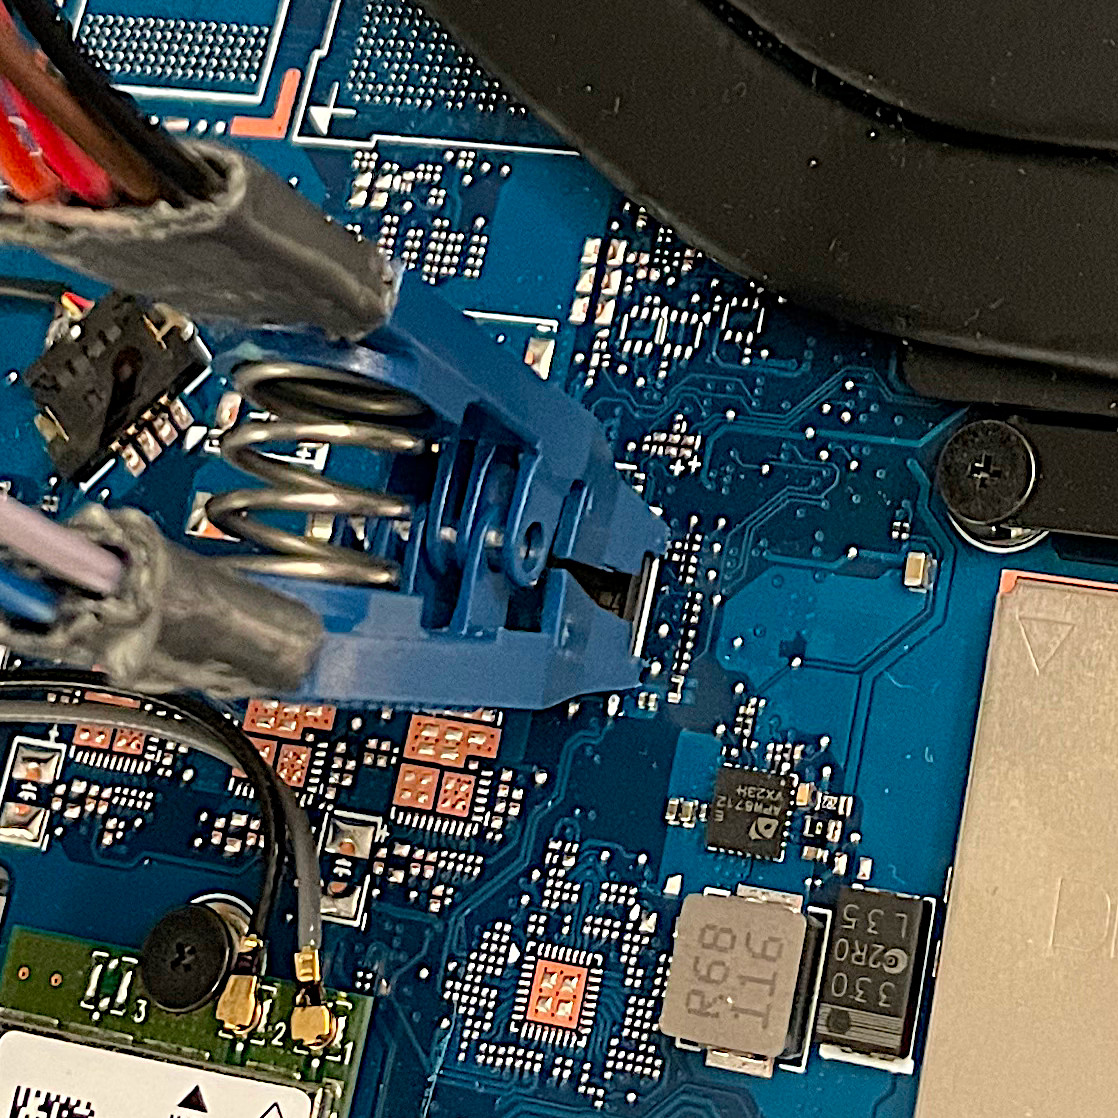
\includegraphics[width=0.75\textwidth]{test-setup/chip-clip}
    \caption{Lenovo Ideapad flash memory accessed with an \acs{SPI} chip clip}
    \label{fig:lenovo-clamp}
\end{figure}

\section{ASRock A520M-HVS}
\label{sec:test-setup:asrock}

Our second hardware setup is a desktop \ac{PC} with an \ac{AMD}\-/based ASRock A520M\-/HVS motherboard.
We use the latest firmware image as of writing, which is version 2.30.
This setup also supports \hyperlink{pcr7-binding}{\ac{PCR}7 binding} when Secure Boot is enabled using the default keys.
The \ac{SPI} flash chip on the main board is disabled and instead an \program{EM100} \ac{SPI} flash emulator is attached.
When the system thinks it is accessing the \ac{SPI} flash chip, it is instead communicating with the emulator.
Additionally, by dual-booting into Linux, we can use \program{flashrom} to communicate with the \ac{SPI} chip directly for read and write access.
The Linux distribution of our choice, Ubuntu, uses a so-called Lockdown Mode when Secure Boot is enabled.
This blocks direct access to the \ac{SPI} chip \cite{man-kernel-lockdown}, but can be disabled while Secure Boot remains enabled \cite{disable-kernel-lockdown}.
